\documentclass[tikz, border=15pt]{standalone}
\usepackage{amsmath}

\begin{document}
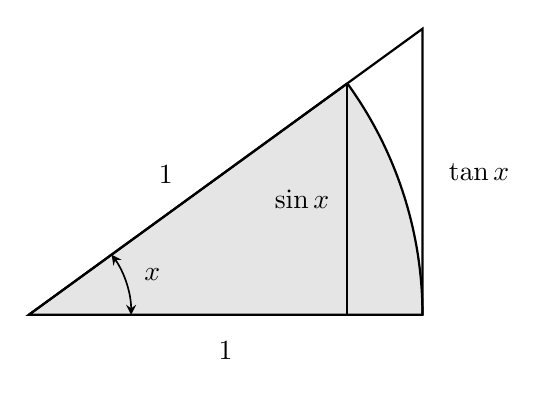
\begin{tikzpicture}[>=stealth]
    % --- 参数定义 ---
    \def\R{5.0}       % 圆半径/底边长度设为 5
    \def\angleX{36}   % 角度设为 36 度

    % --- 1. 填充扇形灰色阴影 ---
    \fill[gray!20] (0,0) -- (\R,0) arc (0:\angleX:\R) -- cycle;

    % --- 2. 绘制主要几何线条 ---
    % 外切直角三角形
    \draw[thick] (0,0) -- (\R,0) -- (\R, {\R*tan(\angleX)}) -- cycle;

    % 扇形圆弧
    \draw[thick] (\R,0) arc (0:\angleX:\R);

    % 斜边半径线
    \draw[thick] (0,0) -- ({\R*cos(\angleX)}, {\R*sin(\angleX)});

    % 内部垂直线 (对应 sin x，加粗增强对比)
    \draw[thick] ({\R*cos(\angleX)}, {\R*sin(\angleX)}) -- ({\R*cos(\angleX)}, 0);

    % --- 3. 标注参数与角度 ---
    % 角度 x 的指示弧与标记
    \def\arcR{1.3}
    \draw[<->, semithick] (\arcR, 0) arc (0:\angleX:\arcR);
    \node at ({(\arcR + 0.35)*cos(\angleX/2)}, {(\arcR + 0.35)*sin(\angleX/2)}) {$x$};

    % 底边长度 1
    \node[below=6pt] at ({0.5*\R}, 0) {$1$};

    % 斜边长度 1 (半径线中点上方)
    \node[above left=2pt] at ({0.5*\R*cos(\angleX)}, {0.5*\R*sin(\angleX)}) {$1$};

    % 内部垂直线长度 sin x (放置在内部线段左侧，避免与弧线重叠)
    \node[left=3pt] at ({\R*cos(\angleX)}, {0.5*\R*sin(\angleX)}) {$\sin x$};

    % 垂直切线长度 tan x
    \node[right=6pt] at (\R, {0.5*\R*tan(\angleX)}) {$\tan x$};

\end{tikzpicture}
\end{document}